\begin{frame}
  \frametitle{Predictions with Random Error}
  \begin{adjustwidth}{-15pt}{0pt}
  \begin{minipage}{0.5\textwidth}
    \begin{figure}
      \centering
      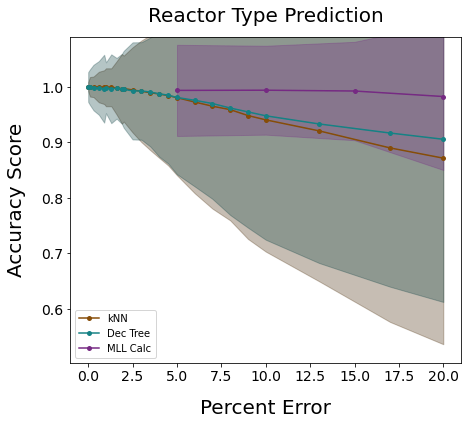
\includegraphics[width=1.03\linewidth]{./figures/randerr_compare_nuc29_rxtr.png}
      \caption{Reactor type prediction (balanced) accuracy using 29 nuclide masses for 3 algorithms}
    \end{figure}
  \end{minipage}%
  \hfill
  \begin{minipage}{0.5\textwidth}
    \begin{figure}
      \centering
      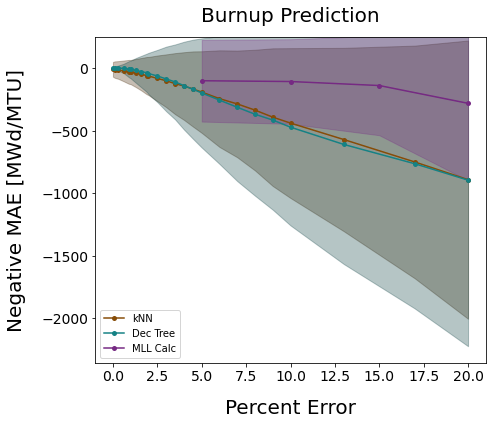
\includegraphics[width=1.08\linewidth]{./figures/randerr_compare_nuc29_burn.png}
      \caption{Burnup mean absolute prediction error using 29 nuclide masses for 3 algorithms}
    \end{figure}
  \end{minipage}
  \end{adjustwidth}
\end{frame}

\begin{frame}
  \frametitle{Predictions with Random Error}
  \begin{adjustwidth}{-15pt}{0pt}
  \begin{minipage}{0.5\textwidth}
    \begin{figure}
      \centering
      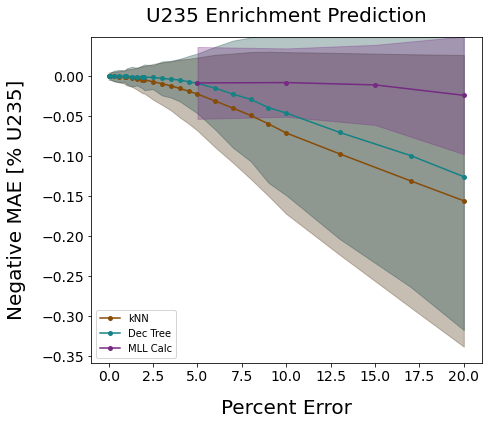
\includegraphics[width=1.08\linewidth]{./figures/randerr_compare_nuc29_enri.png}
      \caption{U235 enrichment mean absolute prediction error using 29 nuclide masses for 3 algorithms}
    \end{figure}
  \end{minipage}%
  \hfill
  \begin{minipage}{0.5\textwidth}
    \begin{figure}
      \centering
      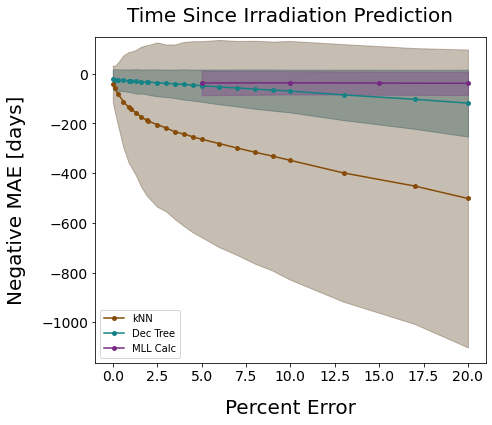
\includegraphics[width=1.08\linewidth]{./figures/randerr_compare_nuc29_cool.png}
      \caption{Time since irradiation mean absolute prediction error using 29 nuclide masses for 3 algorithms}
    \end{figure}
  \end{minipage}
  \end{adjustwidth}
\end{frame}

\begin{frame}
  \frametitle{Predictions of SFCOMPO Test Cases}
  \begin{adjustwidth}{-15pt}{0pt}
  \begin{minipage}{0.85\textwidth}
    \begin{itemize}
      \item 505 test cases in total 
      \item Most test samples have many features missing (see table to left)
      \item Scikit algs don't handle null values, so the missing nuclide measurements are replaced with $0$
    \end{itemize}
    \bigskip
    \begin{table}
      %\centering
      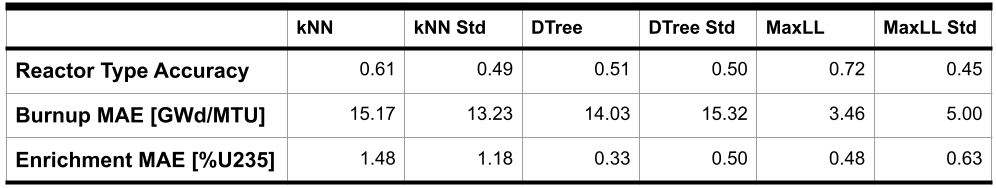
\includegraphics[width=\textwidth]{./figures/sfcompo_pred_results.png}
      \caption{Accuracy (not balanced) and mean absolute errors of the test cases in the SFCOMPO database}
    \end{table}
  \end{minipage}%
  \hfill
  \begin{minipage}{0.15\textwidth}
    \begin{table}
      %\centering
      
\includegraphics[height=0.89\textheight]{./figures/sfcompo_nuc_counts.png}
      %\caption{The number of entries that includes a measurement for each nuclide}
    \end{table}
  \end{minipage}
  \end{adjustwidth}
\end{frame}
